\documentclass{article}

\usepackage{fancyhdr}
\usepackage{extramarks}
\usepackage{amsmath}
\usepackage{amsthm}
\usepackage{amsfonts}
\usepackage{tikz}
\usepackage[plain]{algorithm}
\usepackage{algpseudocode}
\usepackage{amssymb}

\usetikzlibrary{automata,positioning}

%
% Basic Document Settings
%

\topmargin=-0.45in
\evensidemargin=0in
\oddsidemargin=0in
\textwidth=6.5in
\textheight=9.0in
\headsep=0.25in

\linespread{1.1}

\pagestyle{fancy}
\lhead{\hmwkAuthorName}
\chead{\hmwkClass\ (\hmwkClassInstructor\ \hmwkClassTime): \hmwkTitle}
\rhead{\firstxmark}
\lfoot{\lastxmark}
\cfoot{\thepage}

\renewcommand\headrulewidth{0.4pt}
\renewcommand\footrulewidth{0.4pt}

\setlength\parindent{0pt}

%
% Create Problem Sections
%

\newcommand{\enterProblemHeader}[1]{
    \nobreak\extramarks{}{Problem \arabic{#1} continued on next page\ldots}\nobreak{}
    \nobreak\extramarks{Problem \arabic{#1} (continued)}{Problem \arabic{#1} continued on next page\ldots}\nobreak{}
}

\newcommand{\exitProblemHeader}[1]{
    \nobreak\extramarks{Problem \arabic{#1} (continued)}{Problem \arabic{#1} continued on next page\ldots}\nobreak{}
    \stepcounter{#1}
    \nobreak\extramarks{Problem \arabic{#1}}{}\nobreak{}
}

\setcounter{secnumdepth}{0}
\newcounter{partCounter}
\newcounter{homeworkProblemCounter}
\setcounter{homeworkProblemCounter}{1}
\nobreak\extramarks{Problem \arabic{homeworkProblemCounter}}{}\nobreak{}

%
% Homework Problem Environment
%
% This environment takes an optional argument. When given, it will adjust the
% problem counter. This is useful for when the problems given for your
% assignment aren't sequential. See the last 3 problems of this template for an
% example.
%
\newenvironment{homeworkProblem}[1][-1]{
    \ifnum#1>0
        \setcounter{homeworkProblemCounter}{#1}
    \fi
    \section{Problem \arabic{homeworkProblemCounter}}
    \setcounter{partCounter}{1}
    \enterProblemHeader{homeworkProblemCounter}
}{
    \exitProblemHeader{homeworkProblemCounter}
}

%
% Homework Details
%   - Title
%   - Due date
%   - Class
%   - Section/Time
%   - Instructor
%   - Author
%

\newcommand{\hmwkTitle}{Homework\ \#1}
\newcommand{\hmwkDueDate}{September 30, 2017}
\newcommand{\hmwkClass}{Convex Optimization}
%\newcommand{\hmwkClassTime}{Section A}
\newcommand{\hmwkClassInstructor}{Professor Ying Cui}
%\newcommand{\hmwkAuthorName}{\textbf{Josh Davis} \and \textbf{Davis Josh}}
\newcommand{\hmwkAuthorName}{\textbf{Xiaoyi He}}

%
% Title Page
%

\title{
    \vspace{2in}
    \textmd{\textbf{\hmwkClass:\ \hmwkTitle}}\\
    \normalsize\vspace{0.1in}\small{Due\ on\ \hmwkDueDate\ at 11:59pm}\\
    \vspace{0.1in}\large{\textit{\hmwkClassInstructor\ \hmwkClassTime}}
    \vspace{3in}
}

\author{\hmwkAuthorName}
\date{}

%\renewcommand{\part}[1]{\textbf{\large Part \alph{partCounter}}\stepcounter{partCounter}\\}

%
% Various Helper Commands
%

% Useful for algorithms
\newcommand{\alg}[1]{\textsc{\bfseries \footnotesize #1}}

% For derivatives
\newcommand{\deriv}[1]{\frac{\mathrm{d}}{\mathrm{d}x} (#1)}

% For partial derivatives
\newcommand{\pderiv}[2]{\frac{\partial}{\partial #1} (#2)}

% Integral dx
\newcommand{\dx}{\mathrm{d}x}

% Alias for the Solution section header
\newcommand{\solution}{\textbf{\large Solution}}

% Probability commands: Expectation, Variance, Covariance, Bias
\newcommand{\E}{\mathrm{E}}
\newcommand{\Var}{\mathrm{Var}}
\newcommand{\Cov}{\mathrm{Cov}}
\newcommand{\Bias}{\mathrm{Bias}}
\newcommand{\addtag}{\refstepcounter{equation}\tag{\theequation}}

\begin{document}

\maketitle

\pagebreak
% \begin{homeworkProblem}
%     \begin{figure}[h]
%         \centering
%             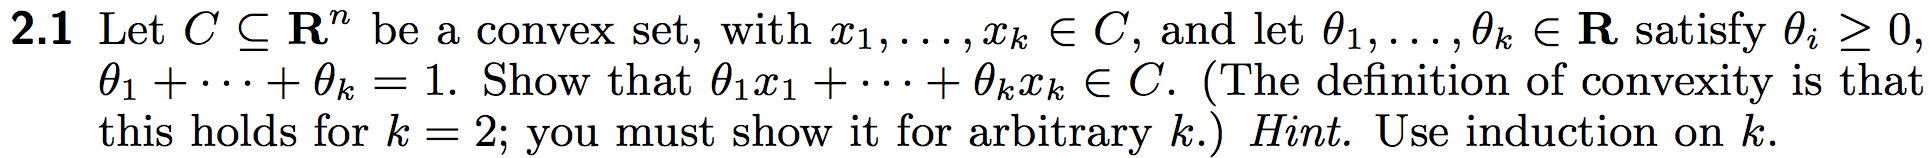
\includegraphics[width=\textwidth]{images/2-1.png}
%     \end{figure}
% \end{homeworkProblem}

\begin{homeworkProblem}
    Textbook Exercises 2.1
    \\

    \begin{proof}
        We use induction on k as the hint said.
        Suppose that the proposition is true when \(k = m - 1 \in \mathbb{R}\) and \(x_{1},\cdots,x_{m} \in C\) and \(\proposition_{1} + \cdots + \theta_{m} = 1\) with \(\theta_{i} \geq 0\). Then we have:
        \[
            y = \theta_{1}x_{1} + \cdots + \theta_{m}x_{m} \tag{1.1} \label{eq:1}
        \]
        we always can find a \(\theta_{r}\) in \(\theta_{1},\cdots,\theta_{m}\) with \(\theta_{r} \neq 1\). So we can get:
        \[
            y = \theta_{r}x_{r} + (1-\theta_{r})(\frac{\theta_{1}x_{1}}{1-\theta_{r}} + \cdots + \frac{\theta_{r-1}x_{r-1}}{1-\theta_{r}} + \frac{\theta_{r+1}x_{r+1}}{1-\theta_{r}} + \cdots + \frac{\theta_{m}x_{m}}{1-\theta_{r}}) \tag{1.2} \label{eq:2}
        \]

        And
        \[
            \frac{\theta_{1}}{1-\theta_{r}} + \cdots + \frac{\theta_{r-1}}{1-\theta_{r}} + \frac{\theta_{r+1}}{1-\theta_{r}} + \cdots + \frac{\theta_{m}}{1-\theta_{r}} = \frac{1-\theta_{r}}{1-\theta_{r}} = 1
        \]
        Also we have that the proposition is true when \(k = m - 1\).
        \[
        (\frac{\theta_{1}}{1-\theta_{r}}x_{1} + \cdots + \frac{\theta_{r-1}}{1-\theta_{r}}x_{r-1} + \frac{\theta_{r+1}}{1-\theta_{r}}x_{r+1} + \cdots + \frac{\theta_{m}}{1-\theta_{r}}x_{m}) \in C
        \]
         Applying the definition of convex set on equation \ref{eq:2}, we can get \(y \in C\). Thus, we can conclude that the proposition is true for arbitrary k. Proof is complete.
    \end{proof}


\end{homeworkProblem}

\pagebreak

\begin{homeworkProblem}
    Textbook exercise 2.8
    \\

    \solution

    (a)Not solved yet.
    \\

    (b)
     S is defined by linear equalities and inequalities. So it is a polyhedra and can be expressed as S where \(A = -1\), \(b = 0\),
    \(F = \left(\begin{array}{c} \mathbf{1}^{T} \\ V_{1}^{T} \\ V_{2}^{T} \end{array} \right)\),
    \(b = \left(\begin{array}{c} 1 \\ b_{1} \\ b_{2} \end{array} \right)\),
    \(V_{1} = (a_{1},\cdots,a_{n})\), \(V_{2} = (a_{1}^{2},\cdots,a_{n}^{2})\)
    \\

    (c) \(x^{T}y \leq 1 \Longrightarrow \Vert x \Vert_{2} \cdot \Vert y \Vert_{2} \leq 1 \), applying \( \Vert y \Vert_{2} = 1\) we get \(\Vert x \Vert \leq 1\). And \(x \succeq 0 \), S is the intersection of \(\{ x \hspace{0.1cm} | \hspace{0.1cm}  \Vert x \Vert_{2} \leq 1\}\) and \(\mathbb{R}^{n}_{+}\). Thus it is not a polyhedra.
    \\

    (d)We have \(x \succeq 0\) and \(\sum^{n}_{i=1} |y_{i}|=1\). So we can proof that:
    \[
        max\left(x^{T}y\right) = max\left(x_{i}\right), i=1,\cdots,n
    \]

    Thus, \(x^{T}y \leq 1 \Longleftrightarrow max\left(x^{T}y\right) = max\left(x_{i}\right) \leq 1 \Longleftrightarrow |x_{i}| \leq 1\), means that S is a polyhedra.

    \[
        x_{i} \geq 0
    \]
    \[
        x_{i} \leq 1
    \]
    \[
        i=1,\cdots,n
    \]



\end{homeworkProblem}

\pagebreak

\begin{homeworkProblem}
    Textbook exercise 2.12 a-e
    \\

    \solution

    (a)It is the solution set of \(\alpha \leq a^{T}x \leq \beta \). Thus it is a polyhedra and convex.
    \\

    (b)the same as (a), so it is convex.
    \\

    (c)the same as (a)(b), so it is convex.
    \\

    (d)
    \[  \begin{split}
        \|x-x_{0}\|_{2} \leq \|x-y\|_{2} &\Longleftrightarrow \left(x-x_{0}\right)^{T}\left(x-x_{0}\right) \leq \left(x-y\right)^{T}\left(x-y\right)
        \\
        &\Longleftrightarrow x^{T}x - 2x_{0}^{T}x + x_{0}^{T}x_{0} \leq x^{T}x - 2x_{i}^{T}x + x_{i}^{T}x_{i}
        \\
        &\Longleftrightarrow 2\left(x_{i}-x_{0}\right)x \leq x_{i}^{T}x_{i} - x_{0}^{T}x_{0}
        \end{split}
    \]
    It is a halfspace given a fixed \(y \in \mathbb{C}\). So the set is the intersection of multi-halfspace and thus it is convex.
    \\

    (e)It is not convex.
\end{homeworkProblem}
\pagebreak

\begin{homeworkProblem}
    Textbook exercise 2.15
    \\

    \solution

    (a)The set is solution set of two linear inequalities so it is convex.
    \\

    (b)We set \(a_{r}\) is the minimum one that great than \(\alpha\).
    \[
        \mathbf{prob}\left(x > \alpha\right) \leq \beta \Longleftrightarrow \sum_{i=r}^{n} p_{i} \leq \beta
    \]

    Thus, it is  convex.
    \\

    (c)
    \[
        \begin{split}
            \mathbf{E}|x^{3}| \leq \alpha \mathbf{E} |x| &\Longleftrightarrow \sum_{i=1}^{n}|a_{i}^{3}|p_{i} \leq \alpha \sum_{i=1}^{n}|a_{i}|p_{i}
            \\
            &\Longleftrightarrow \sum_{i=1}^{n}\left(|a_{i}^{3}|-\alpha|a_{i}|\right)p_{i} \leq 0
        \end{split}
    \]
    Thus, the set is convex.
    \\

    (d)
    \[
        \mathbf{E}x^{2} \leq \alpha \Longleftrightarrow \sum_{i=1}^{n}x^{2}p_{i} \leq \alpha
    \]
    Also convex.
    \\

    (e) similar with (d), this condition also define a convex set.
    \\

    (f)
    \[
        \mathbf{var}\left(x\right) \leq \alpha \Longleftrightarrow \sum_{i=1}^{n}a_{i}^{2}p_{i}-\left(\sum_{i=1}^{n}a_{i}p_{i}\right)^{2} \leq \alpha
    \]

    We can take \(n = 2, a_{1} = 1, a_{2} = 0\).The condition becomes:
    \[
        p_{1}-p_{1}^{2} \leq \alpha
    \]
    If we take \(\alpha = \frac{1}{6} \), \(p^{1} = \left(1,0\right)\), \(p^{2} = \left(0,1\right)\) and \(p^{3} = \frac{1}{2}p^{1} + \frac{1}{2}p^{1} = \left(\frac{1}{2},\frac{1}{2}\right)\), we can get:
    \[
        p_{1}^{1} - \left(p_{1}^{1}\right)^{2} = 0 \leq \alpha = \frac{1}{6}
    \]
    \[
        p_{1}^{2} - \left(p_{1}^{2}\right)^{2} = 0 \leq \alpha = \frac{1}{6}
    \]
    \[
        p_{1}^{3} - \left(p_{1}^{3}\right)^{3} = \frac{1}{4} \geq \alpha = \frac{1}{6}, p^{3} \notin set P
    \]

    Thus,it is not convex.
    \\

    (g)

    \[
        \mathbf{var}\left(x\right) \leq \alpha \Longleftrightarrow \sum_{i=1}^{n}a_{i}^{2}p_{i}-\left(\sum_{i=1}^{n}a_{i}p_{i}\right)^{2} \geq \alpha \tag{4.1} \label{eq:4.1}
    \]
    We can take \(p^{1},p^{2}\) that satisfy equation \ref{eq:4.1}, i.e:
    \[
        \sum_{i=1}^{n}a_{i}^{2}p_{i}^{1}-\left(\sum_{i=1}^{n}a_{i}p_{i}^{1}\right)^{2} \geq \alpha
    \]
    \[
        \sum_{i=1}^{n}a_{i}^{2}p_{i}^{2}-\left(\sum_{i=1}^{n}a_{i}p_{i}^{2}\right)^{2} \geq \alpha
    \]
    And we take \(p^{3} = \theta_{1}p^{1} + \theta_{2}p^{2}\), where \(\theta_{1}+\theta_{2} = 1\) and \(\theta_{1},\theta_{2} \in [0,1]\).
    \[
        \begin{split}
        \sum_{i=1}^{n}a_{i}^{2}p_{i}^{3}-\left(\sum_{i=1}^{n}a_{i}p_{i}^{3}\right)^{2} &= \theta_{1}\sum_{i=1}^{n}a_{i}^{2}p_{i}^{1}+\theta_{2}\sum_{i=1}^{n}a_{i}^{2}p_{i}^{2}+ \left(\theta_{1}\sum_{i=1}^{n}a_{i}p_{i}^{1} + \theta_{2}\sum_{i=1}^{n}a_{i}p_{i}^{2}\right)^{2}
        \\
        & \geq \theta_{1}\sum_{i=1}^{n}a_{i}^{2}p_{i}^{1}+\theta_{2}\sum_{i=1}^{n}a_{i}^{2}p_{i}^{2}- \theta_{1}\left(\sum_{i=1}^{n}a_{i}p_{i}^{1}\right)^{2} - \theta_{2}\left(\sum_{i=1}^{n}a_{i}p_{i}^{2}\right)^{2}
        \\
        & \geq \theta_{1}\alpha + \theta_{2}\alpha
        \\
        & = \alpha
        \end{split}
    \]
    Thus, \(p^{3} \in \mathbf{P}\). The set is convex.
    \\

    (h)\(\mathbf{quartile}\left(x\right) \geq \alpha\) is equivalent to:
    \[
        \mathbf{prob}\left(x \leq \beta\right) \geq 0.25, \mbox{for all } \beta \geq \alpha \Longleftrightarrow \mathbf{prob}\left(x \leq \beta\right) \leq 0.25, \mbox{for all } \beta < \alpha
    \]
    We can define \(a_{k} = max\left\{a_{i} | a_{i} < \alpha\right\}\),then:
    \[
        \begin{split}
        \mathbf{prob}\left(x \leq \beta\right) \leq 0.25, \mbox{for all } \beta \geq \alpha &\Longleftrightarrow \mathbf{prob}\left(x \leq \beta_{max}\right) \leq 0.25
        \\
        &\Longleftrightarrow \mathbf{prob}\left(x \leq a_{k}\right) \leq 0.25
        \\
        &\Longleftrightarrow \sum_{i=1}^{k}p_{i} \leq 0.25
        \end{split}
    \]
    It is a halfspace and convex.
    \\

    (i)Similar with (h), this condition is equivalent to:
    \[
        \mathbf{prob}\left(x \leq \alpha\right) \geq 0.25 \Longleftrightarrow \sum_{i=1}^{k}p_{i} \geq 0.25
    \]

\end{homeworkProblem}



\end{document}
